%file included in thesis.tex

\chapter{Implementation}
\label{chap6}
In this chapter implementation specific issues are treated. Figure
\ref{chap6:fig-implementation} shows the three-layer implementation of the project.
\begin{figure}[htbp]
    \centering
    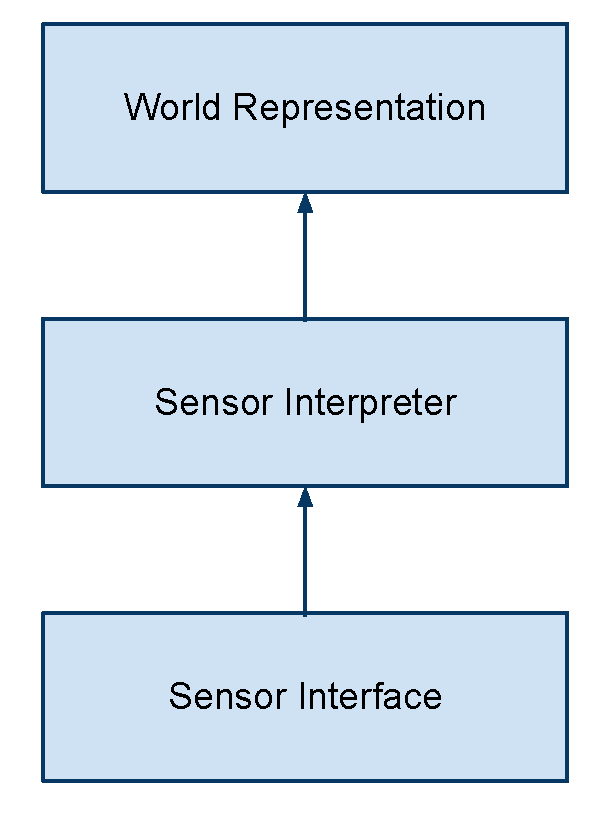
\includegraphics[width=0.4\textwidth]{pics/implementation}
    \caption{Three-layer implementation}
    \label{chap6:fig-implementation}
\end{figure}
The \emph{low-level} layer reads and converts the raw sensor data into common data which can be
interpreted by the \emph{middle} layer. This layer handles all the ''washing`` of the
sensor data, and applies the reasoning and tries to recognize the environment. The third
and last layer is the \emph{world} layer which handles the global data, where the robot is
and where it should move next. 

The project is implemented in both \emph{C/C++} and Matlab. The sensor layer are
implemented in \emph{C/C++} while the other layers are implemented in Object-Oriented
Matlab.

\section{Low-level Interfaces}
The low-level interfaces from the sensors are implemented in \emph{C/C++} and uses the
supplied sensor APIs. The SwissRanger 3000 API were used directly in Matlab. The Hokuyo
API was a little more tricky to use. A Matlab interface function were implemented to get
the sensor data directly into Matlab.

\subsection{Hokuyo URG Sensor Interface}
A sensor API for \emph{C/C++} was supplied from the manufacturer of the laser range
finder. Standard API calls were used and a precompiled matlab \emph{mex}-file was created
for sensor access from matlab. The code can be seen in Appendix \ref{app:urg-mex}.

\subsection{SwissRanger 3000 Sensor Interface}
MESA Imagining provided a standard matlab interface with the needed functionality, and
were generally plug-and-play, using the \emph{sr\_aqquire()} to tell the camera to get
ready for capture. \emph{sr\_getimage()} where used to get the intensity image, while
\emph{sr\_coordtrf()} gave the Cartesian coordinate output. Default integration time for
the camera where used. 

\subsection{Stereo Camera Implementation}
For the stereo camera, a program was written using the \emph{OpenCV} library. A open
source computer vision library, initially developed by Intel. This library have many
excellent and optimized functions for grabbing images, camera calibration, image rectification
and stereo matching. This produced a disparity map, which again where reprojected into 3D
by the \emph{cvReprojectTo3D()}-function. This coordinate images where saved to disk and
read into Matlab for further processing. 

\begin{algorithm}
\caption{The Stereo Capture Procedure}
\label{chap6:alg-stereomatch}
    \begin{algorithmic}
    \STATE \textbf{begin}
    \STATE Connect to Cameras
    \FOR{no of images $<$ 20}
        \STATE Capture images of Checkerboard and find corners
    \ENDFOR
    \STATE Calculate the distortion parameters using Healy's Method.
    \WHILE{Not Quitting}
        \STATE Capture images
        \STATE Rectify Images
        \STATE Stereo matching using Block Matching 
        \STATE Reproject disparity map to 3DImage
        \STATE Dump 3D Coordinates to Disk
    \ENDWHILE
    \STATE \textbf{end}
    \end{algorithmic}
\end{algorithm}
This program calibrates the cameras, rectifies the images, finds stereo correspondences
and reprojects them to 3D coordinates. The source code is shown in Appendix
\ref{app:dense-stereo}.


\section{Mid-level Implantations}
The middle layers goal is to process and interpret the sensor data to best ability. This
layer is in charge of doing the reasoning, and draw out important information form the
sensor data. The main task is to find lines in the 2D sensor data, and cylinder shapes in
the 3D data. 

This functionality are implemented in a Matlab class called the \emph{SensorInterpreter}.
The m-file is given in the Appendix \ref{app:sensorinterpreter}. The implementation is
straight forward and brute force. 


\subsection{Analysis of 3D Sensor Data}
The algorithm which is used is the \emph{EUROMETROS}\cite{eurometros} Matlab library developed by
\emph{National Physics Laboratory(NPL)} in the United Kingdom. The algorithm provides the
estimated radii, and directions of the data sets. Also the distance of the data set to the
estimated cylinders are output, which is a measurement on how good the cylinder fit is. 


\section{High-level Implementations}

\subsection{World Representation}
The world representation are implemented as objects in Matlab. Each node in the world
representation described in Chapter \ref{chap5} are implemented as a class in Matlab. 
\begin{figure}[htbp]
    \centering
    %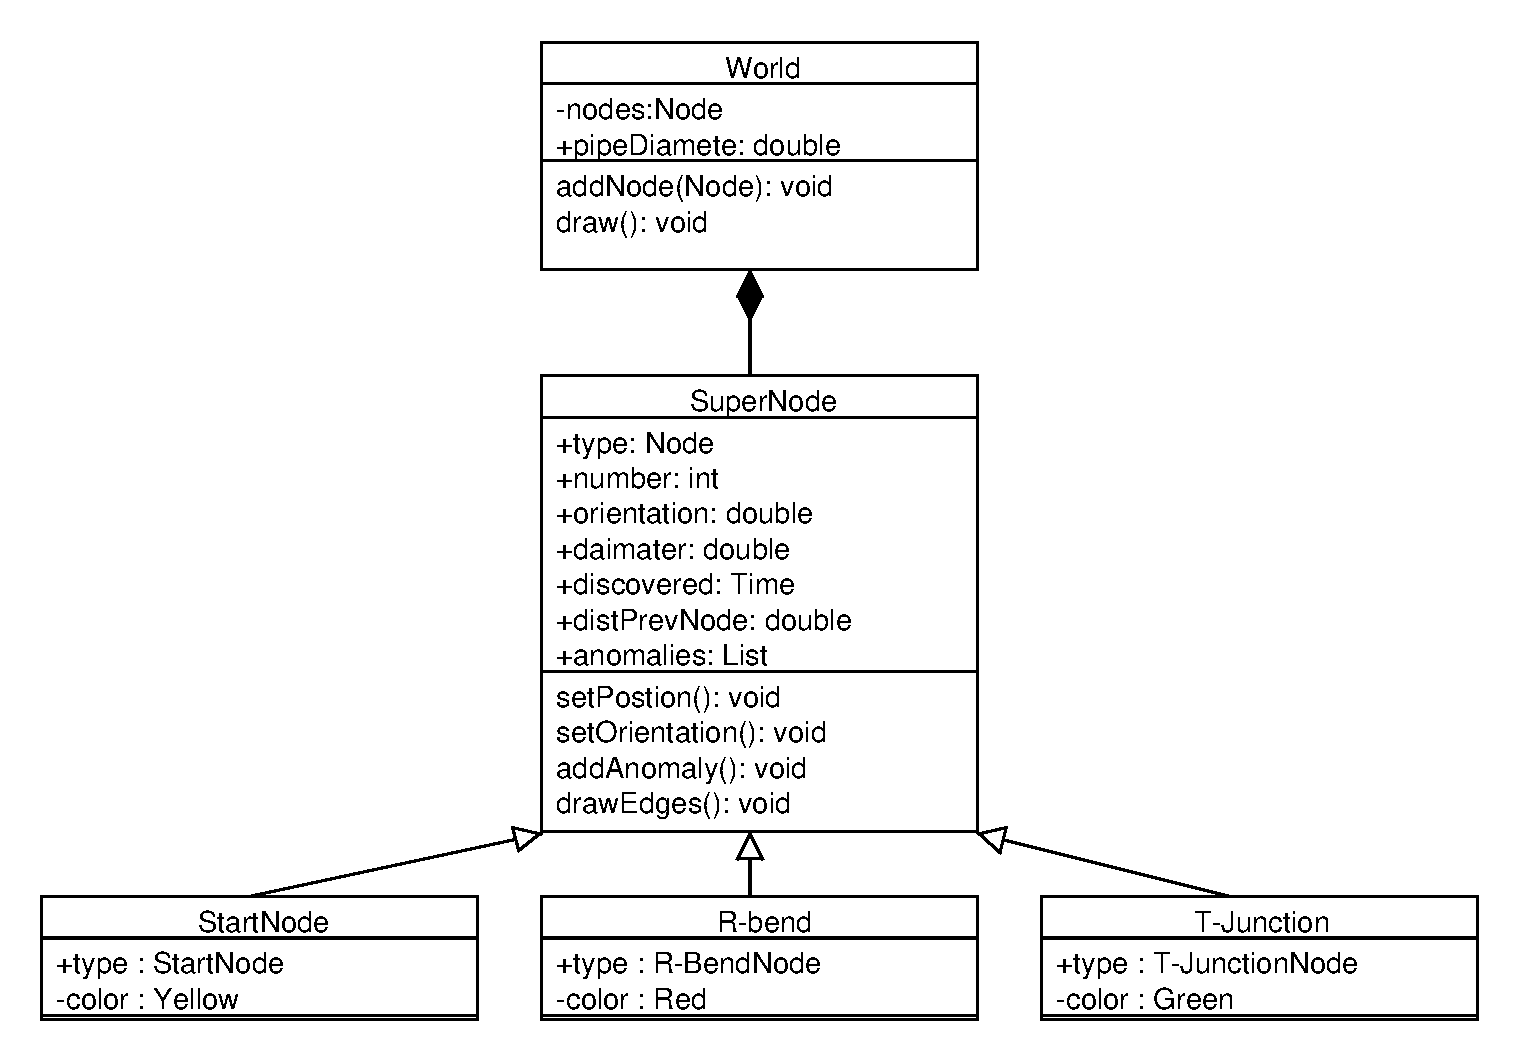
\includegraphics[width=0.6\textwidth]{pics/world-uml}
    \caption{UML of the world representation}
    \label{chap6:fig-world-uml}
\end{figure}

As seen from Figure \ref{chap6:fig-world-uml} the implementation are based on a
\emph{world} class which contains the á priori map of the world and the node network
together with some useful parameters. The nodes of the representation are also different
classes which inherits from a super node. See Appendix \ref{app:world} for the matlab
code. 


\section{Summary of Parameters}
Here a summary of the different parameters that the user is required to set, and guess, is
given. 
\begin{table}[htbp]
    \centering
    \begin{tabular}{|r|l|}
        \hline
        $LowIntensity$ &  Threshold value for filtering low intensity pixels   \\
        $HighIntensity$ & Threshold value for filtering high intensity pixels  \\
        Interval      &  The interval for which the point cloud should be divided \\
        $m$             &  value which defines $m r_i$ as errenous             \\
        \hline
        $hits_y$    &  The bin sizes of the histogram in the y direction       \\
        $hist_x$    &  The bin sized of the histogram in the x direction       \\
        $NoPointsY$ &  The number of points in a bin to define a line          \\
        $NoPointsX$ &  The number of points in a bin to define a line         \\
        $P_1$       &  The distance of the measurement plane of the URG in meters\\
        $ParallelThreshold$ &  Upper value that defines if two lines are parallel \\
        \hline
        $NoChessBoardImages$ & images of the checkerboard required for stereo camera calibration         \\
        \hline
    \end{tabular}
    \caption{Summary of the user parameters}
    \label{chap6:tab-user-parameters}
\end{table}

\section{What is not Implemented}
There are a number of things that are not implemented because of time issues. Probably the
most important thing is the segmentation of the sensor data. This is crucial for the
least-squares method to work properly. 

Depth calibration of the Time-of-flight camera are not implemented, due to the reasons
given in Section \ref{chap3:subsec-depht-calib}.

The module that recognizes and matches pipe profiles are not implemented. 
The idea of this is that it will from the sensor interpreter recognize the pipe
profile, which is matched to some internal database of profiles.

Also, the matching algorithm for finding the global position from the passed-through nodes
have also been skipped for time issues. All, of this modules are easy to insert in the
present implementation, because of the modular architecture. 


